\documentclass[twoside,12pt,titlepage]{article}
\usepackage{setspace}
\usepackage[pdftex]{graphicx}
\usepackage[margin = 1in]{geometry}
\usepackage{enumitem}
\usepackage{amsmath}
\usepackage{siunitx}
\usepackage{fancyhdr}
\usepackage{chemmacros}
\setlength{\headheight}{15pt}

\newcommand{\machen}{Michael A. Chen}
\newcommand{\isotope}[2]{\ch{^{#1}#2}}
\pagestyle{fancy}
\lhead{\machen}
\chead{Thesis Proposal}
\rhead{\today}
\cfoot{\thepage}

\title{Studies of radioisotopes for use \\as tracers in groundwater systems}
\author{\machen}

\begin{document}
\maketitle
\thispagestyle{plain}

\begin{abstract}
Words
\end{abstract}

\section{Introduction}

In the past 100 years, radionuclides have become intimately tied with human society, serving as fuel sources, weapons, and tracers for both medical and environmental processes. Despite their ever increasing ubiquity, there is a strained relationship with these compounds, one often characterized by distrust and fear \cite{Hohenemser1977}. As one example, the 2011 Fukushima Dai-ichi Power Plant accident has driven some countries to abandon nuclear energy programs all together in attempt to avoid releases of nuclear material that could occur due to unforeseen circumstances. In parallel however, nuclear energy and medicine are still used globally \cite{Ramana2013}, and their waste products require careful treatment and disposal. One subject area requiring significant more understanding is the transport of these waste products in groundwater systems. As seen by the continuing work at the Savannah River, poor management of waste can lead to persistent contamination of groundwater \cite{Emerson2014}. Groundwater transport also plays an important role in the fate of contaminants at Fukushima, though many radioisotopes require further study \cite{Steinhauser2014}.
\par Among these radioisotopes, two elements stand out: Radium and Iodine. Radium has multiple isotopes that are naturally occurring in the environment, with a range of half-lives from a few weeks to thousands of years. While it has seen usage in the past in as a dubiously safe popular medicine, and as a luminescent compound, it currently sees little commercial usage \cite{WikiRadium}. Radium’s societal relevance comes not from its commercial usage, but from natural settings. Brines sourced from shales, which are sources for hydrocarbons used in hydraulic fracturing, or "fracking"', operations can contain up to \SI{0.7}{\nano Ci\per\liter} of Radium \cite{Barbot2013}, and must be carefully managed. Radium also has been identified as a key natural tracer for groundwater discharge into the ocean, where the natural background generation of radium isotopes is by thorium and uranium \cite{Moore2000}. Characterization of radium isotope transport properties similar to that of \isotope{137}{Cs} \cite{Steinhauser2014} is crucial toward using those isotopes in accurate transport based estimates of groundwater flow. 
\par The literature is peppered with a number of sources discussing the behavior of radium on solids. There were a number of studies measuring radium sorption on to various solids such as ferrihydrite, muscovite, and natural estuarine sediments, reporting a wide range of distribution coefficients \cite{Ames1983a,Ames1983b,Benes1984}. These studies formed a basis for understanding radium sorption behavior, but did not address the mechanisms of sorption or surface complexation. Later studies included other sediments \cite{Tachi2001} and radium saw the beginnings of its current usage as a groundwater tracer \cite{Moore1996}. Recent studies focusing on marine sediments compiled earlier work, finding huge variability in radium $K_d$ values, ranging from \SI{1.2}{\liter\per\kilo\gram} to \SI{38000}{\liter\per\kilo\gram}, with orders of magnitude variation occurring even with similar media and sorbent \cite{Beck2013}. There has been little study of radium in shale brines sourced by hydraulic fracturing outside of pure characterization \cite{Barbot2013,Rowan2011}. Thus there clear gaps in understanding radium behavior in fracking conditions as well as its surface complexation behavior.
\par Iodine is another element of interest with one naturally abundant, stable isotope, \isotope{127}{I}, and a few radioactive isotopes, \isotope{129}{I} and \isotope{131}{I}, whose major sources are anthropogenic nuclear activity \cite{He2013,Landis2012}. \isotope{127}{I} is a crucial micronutrient for human life that is found primarily in thyroid proteins \cite{Hu2009}. \isotope{129}{I} and \isotope{131}{I} are both radioactive isotopes that can be incorporated into the thyroid, leading to thyroid cancer, presenting a significant health risk during nuclear release accidents. Understanding its transport in soils and groundwater is thus crucial for both the maintenance and protection of human health. Additionally, the long half-life of \isotope{129}{I} and its low natural abundance suggest that it could be used as a tracer for nuclear material release \cite{He2013}. However, efforts to understand its transport are complicated by complex speciation behavior.
\par Iodine has a multitude of oxidation states, partitions significantly into organic matter, and can be volatile at environmental conditions, all of which affects its transport and speciation in groundwater systems. Fortunately, the only primary oxidation states for iodine in environmental systems are elemental iodine, \ch{I2}, iodide, \ch{I-}, and iodate, \ch{IO3-} \cite{Hou2009}. A figure illustrating these oxidation states can be seen in figure \ref{fig:IodineSpeciation}. Iodine also partitions into organic matter and there is evidence for both biotic and abiotic mechanisms for the incorporation of inorganic iodine into organic molecules \cite{Gilfedder2010, Yamaguchi2008}. Iodine cycling with respect to organic matter still has many unresolved questions, including the dominant mechanisms, and where those mechanisms come into play. Some of the iodine bearing organic compounds and elemental iodine are volatile, and can degas and escape from soils \cite{Hu2009}. Given the wide variety of forms iodine can take in a given system, significant effort has been made toward analytical tools to separate different forms of iodine. Common techniques take advantage of a chromatographic methods, such as high pressure liquid chromatography (HPLC) in combination with a ICP-MS to study iodine speciation \cite{Wuilloud2005}. Recent studies of transport behavior have leveraged these tools to study the behavior of the inorganic, aqueous iodine species and representative organoiodine compounds in specific media \cite{Hu2005}. Batch sorption experiments showed that iodine sorption is relatively weak to clay minerals, but stronger in the presence of reduced metal oxides and sulfides, and is almost entirely dominated by the presence of organic matter \cite{Assemi1994,Fuhrmann1998}. Similarly, there is not a clear understanding of even the basic kinetics and mechanisms of iodine incorporation into organic matter, nor is there strong understanding of the subsuquent transformation and release of those iodine species from organic matter, both biotically and abiotically \cite{Yamaguchi2008,Kaplan2014}. Careful characterization of these processes would enable iodine usage as a tracer for anthropogenic nuclear activity.

\begin{figure}
\centering
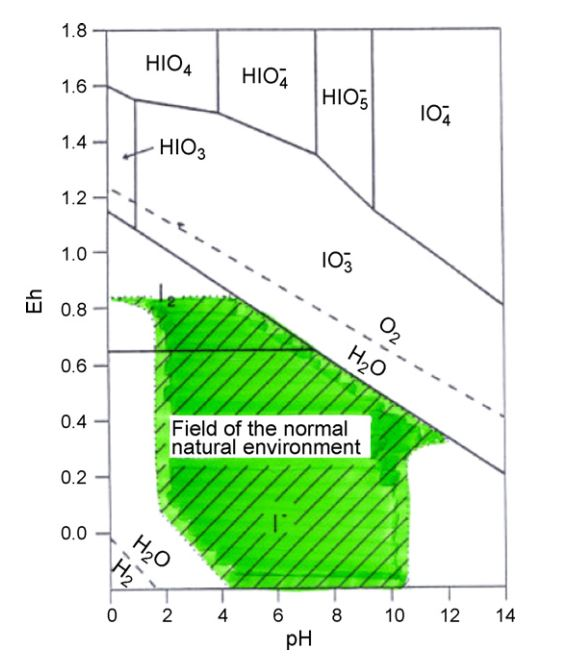
\includegraphics[width = 0.4\textwidth]{IodineSpeciation.png}
\caption{Eh-pH diagram for iodine in water at \SI{25}{\degreeCelsius}, with highlighting of common environmental conditions from \cite{Hou2009}.}
\label{fig:IodineSpeciation}
\end{figure}

\section{Objectives}

A common theme in studies of radium and iodine is developing or improving their functionality as environmental tracers in natural ground and surface waters. To this end, I broadly propose work that would serve to improve, augment, or enable their usage as tracer environmental tracers by developing specific understanding of the mechanisms controlling their transport and speciation.
\subsection{Radium}

\begin{enumerate}[label=\arabic*)]
	\item Radium transport in groundwater is dominated by a handful of minerals, and I expect it will be possible to build an accurate model of groundwater flow by accounting for these dominant minerals. I expect oxidized minerals, particularly iron and manganese oxides, to be prominent, if not the primary sorbing phases in environmental systems.
	\item I expect that in situ transformation from reduced minerals to oxidized minerals, or between oxidized mineral phases (as an example, ferrihydrite to goethite or hematite) will result in dynamically varying transport conditions for radium.
	\item I hypothesize that given radium's usage as a tracer in groundwater flow, and its elevated concentrations in produced water, it will be possible to trace surface water contamination resulting from improper storage of hydraulic fracturing wastes.
\end{enumerate}

\subsection{Iodine}

\textbf{\cite{Fuhrmann1998} completely changes everything (since they did a lot of the inorganic work), should restructure this along those lines, in addition, investigate further work by that group, and previous work. Is there consistency between various estimates for iodine sorption to these minerals? Also, may want to discuss potential for a field campaign in Hawaii as a model system for studying iodine cycling through organic phases, using either Fukushima or weapons testing on Johnston atoll as a tracer pulse}

\begin{enumerate}[label = \arabic*)]
	\item In spite of the complex iodine interactions with organic matter, it should be feasible to establish some basic parameters to establish constraints on iodine transport in the presence of organic matter. To this end, I would seek to characterize iodine sorption and transformation in organic matter, focusing on how organic matter composition, organic matter concentration, and system oxidation state affect those transport properties. I would focus on the fixation of iodine to organic molecules and brought on by contact with organic matter as important transformations.
	\item A second confounding factor on understanding iodine transport are the controls on its speciation, thus I seek to study how both organic matter, and inorganic minerals control that speciation. I expect in situ reduction and oxidation of minerals, particular iron and aluminum oxides that are stronger inorganic sorbents of iodine species, can be paired with oxidation and reduction of iodine species, controlling directly iodine speciation, and indirectly, iodine species transport properties.
\end{enumerate}



\section{Proposed Research}

Given the large differences in the transport behavior of radium and iodine, work will be split along element specific sets of studies.

\subsection{Radium}

\subsubsection{Sorption Studies}
The first step in understanding radium transport behavior is to study basic Radium sorption behavior, using batch experiments with a single mineral in well controlled environments, using an appropriate isotope. Currently, I am using \isotope{226}{Ra}. Because of radium's $2+$ oxidation state and the few previous studies of radium sorption, I expect the major controlling element to be iron. As a result I plan to study, at minimum, the following minerals:

\begin{itemize}
	\item Ferrihydrite
	\item Pyrite
	\item Quartz
	\item Smectite
\end{itemize}

\par Ferrihydrite is a dominant environmental sorbent, often being the dominant sorbing phase in a given soil. \textbf{MORE EXPLANATION}
\par There are previously established methods of making these minerals, or they can be purchased. Reduced minerals, like pyrite can form oxidized coatings \cite{Buckley1987}, so experiments with these minerals need to be performed anaerobically, while oxidized minerals can be used in normal lab conditions. Minerals that I make can be standardized for iron content by either digestion and analysis with an inductively coupled plasma mass spectrometer (ICP-MS), or through colorimetric methods \cite{Viollier2000}. Minerals that are made will also be taken to synchrotron facilities for structural analysis, using x-ray absorption near edge structure (XANES) and x-ray absorption fine structure (EXAFS) techniques \cite{Fendorf1999}. These methods can be used to confirm the mineral structures expected, as well as grant insight into sorptive behavior.
\par The second part of these batch experiments is controlling the solution that radium partitions into. Given the current lack of sorption data regarding radium, the media will be:

\begin{enumerate}[label = \roman*)]
	\item Pure water
	\item Artificial groundwater
	\item Artificial seawater
	\item Shale brine or equivalent high ionic strength solution
\end{enumerate}

Groundwater and seawater are common environmental media for subsurface settings, with some systems having both mixing. There are well established recipes for artificial groundwater and seawater such as those provided by ASTM \cite{ASTMSeawater2013}. It may be possible to use samples of groundwater or seawater from specific targeted sites for a more site specific characterization. Unfortunately, there isn't an established recipe for artificial brine, and access to natural shale brines may be limited by the companies running the natural gas extraction sites. These brines contain huge amounts of dissolved salts, an average of \SI{106390}{\milli\gram\per\liter} total dissolved solids (TDS), and exist at significantly different temperatures and pressures compared to seawater or groundwater. Thus I expect a major confounding factor in formulating a characteristic artificial brine will be preventing precipitation of various solids. Despite this, I expect to be able to create a representative, high ionic strength medium that is comparable to a shale brine, which can be used in these experiments. It may also be worthwhile to perform some of these experiments at elevated temperature, to better approximate the in-situ conditions in a shale.

\par In addition to variations in the media and mineral, I plan to perform a few types of batch sorption experiments. The first is a set of simple 24-hour sorption experiment, which I have already begun using \isotope{226}{Ra} and FHY in pH \num{3.5} water, whose preliminary results are shown in figure \ref{fig:RaFHYSorb}. The next experiment type is a time based sorption study, looking at the kinetics of the sorption process, as well as establishing an equilibration time for short term sorption processes. This experiment may need to run longer than 24 hours if I see variations in the sorptive behavior over longer times. The results of these experiments may help update the other possible experiments by giving a more accurate window of time for when equilibration occurs. The last set of experiments will be surface complexation studies, where the pH of the experiment is strictly controlled, which allows for a better understanding of the processes controlling radium sorption to these minerals.

\begin{figure}
	\centering
	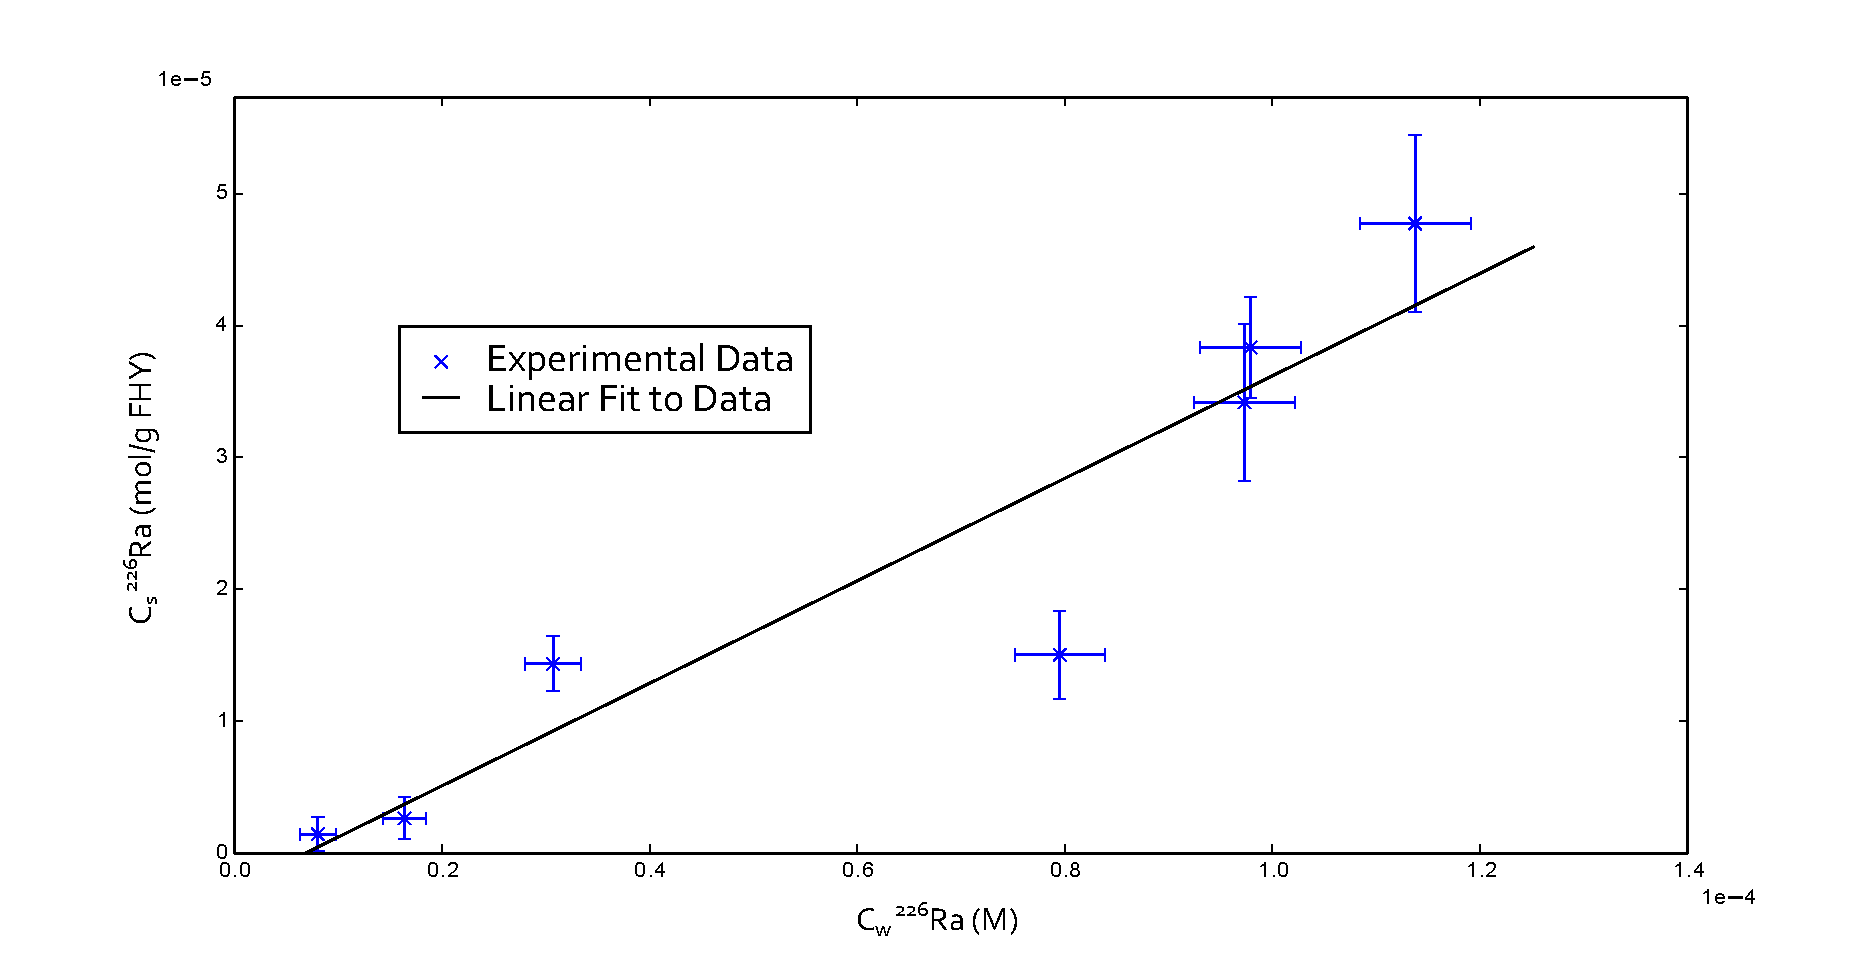
\includegraphics[width=0.8\textwidth]{AGU2014FHYRa.pdf}
	\caption{Figure showing preliminary sorption of \isotope{226}{Ra} to FHY in water at pH \num{3.5}. Error bars represent analytical uncertainty, and the linear fit is a simple polynomial fit using a NumPy polynomial fitting function. The fit gives a partition coefficient of \SI{0.39}{\liter\per\gram}.}
	\label{fig:RaFHYSorb}
\end{figure}

\par The data produced by these experiments provide the groundwork for modeling the sorption behavior of radium on these minerals. Fitting the equilibrated batch sorption experiments to a Langmuir or Freundlich type isotherm provides coefficients that can be used to predict solid-solution behavior in groundwater systems. This can be accomplished using a basic numerical tool such as the python package NumPy or more specialized software such as PHREEQC \cite{PHREEQC}. The time series experiments can be used to establish a foundational sense of the kinetics of radium sorption, examining how quickly equilibration can be reached. Lastly, the results of the pH controlled experiments can be fitted to build a surface complexation model that builds a picture of radium behavior on the surface of the various minerals, which can be accomplished with transport modeling software like PHREEQC or specialized tools \cite{Dixit2003}. This behavior can then be examined in further detail at synchrotron facilities by using XAFS and XANES methods on minerals with sorbed radium. This suite of models and fits will build a more complete picture of radium surface behavior, as well as help establish what minerals are dominant in controlling radium transport.

\subsubsection{Transport Studies}

The next logical step in studying the transport behavior of radium in groundwater is to run small scale column studies under well controlled conditions, which take advantage of the previously studied sorptive behavior, which would be used to understand how radium is carried by groundwater in various conditions. The general procedure would be to pack columns of an inert porous media (such as glass beads, or quartz sand) would be packed with a known, well distributed quantity of a particular mineral of interest, which would have been previously studied. Flow of some water, be it pure water or a brine, would be pushed through the column containing a known concentration of radium, and measurements of the effluent from the column would be analyzed for radium concentrations. Variations in the timing, initial condition, and the constituents of these columns can be controlled to analyze different phenomena.
\par Initial phenomena I would wish to study is importance of sorption on the transport of radium in these columns. To study this, I would perform a series of column experiments containing increasing amounts of a sorbing mineral such as ferrihydrite. In one set of experiments, I would saturate the column with a solution contianing no radium, and then flow a solution containing a known concentration of radium through the column. The effluent of the column would be sampled for radium until the effluent concentration reaches a steady state condition. After this, I would then flow a solution without radium through, again sampling the effluent and measuring for radium until some steady state is reached. These time based experiments would establish a number of radium transport properties in ideal conditions. These include, typical breakthrough times, equilibration times, retardation factors, and the strength of radium retention. Variations of the mineral and solution composition, similar to that in the sorption experiments would further elucidate important factors in transport. These experiments in ideal conditions would then give way to experiments in less ideal conditions, using more complicated media and solutions. For example, soil cores from relevant field sites, such as those near Fukushima, or other field sites such as those at the Massachusetts Military reservation on Cape Cod can be used \textbf{CITE SOMETHING PLEASE}.
\par These column experiments would also be accompanied by modeling efforts using transport modeling software PHREEQC and MIN3P \textbf{CITATION?}, which would be calibrated to predict the characteristic behavior of the experiments. To do this, data from the sorption experiments will be combined with measurements of the column characteristics (such as porosity) to produce concentration profiles over time. A properly calibrated model will closely match the experimental results. Ideally, I would prefer to avoid generating empirical parameters for these model fits, as they will have little value when evaluating real life situations with more complex porous media.
\par One other column experiment of interest is one in which I attempt to alter the minerals present in the column itself by the introduction of an oxidizing agent, such as potassium permanganate. For example, pyrite, a reduced iron mineral, could be oxidized to induce additional sorption of radium. These experiments would be operated in a similar manner as the simpler column experiments, but would involve tracking both amounts of radium and the oxidizing agent. Columns may also be run using only the oxidizing agent, and the resulting porous media may be sampled and taken to a synchrotron to analyze what minerals have formed. These experiments could be modeled as well, though more effort would be applied to establishing if these transformations would be useful and feasible for controlling radium transport in field settings.

\subsubsection{Field Campaign}
Given the heightened risks of radium contamination as a result of hydraulic fracturing work, it is important to gather data on whether or not hydraulic fracturing operations are causing contamination of local surface water. To this end, I would propose a field campaign in northwestern PA, in one of the national forest regions, such as Allegheny National Forest to collect data on water quality near fracturing wells. These types of regions are ideal for this work, as the potentially affected watersheds sit on open access land, yet have a plethora of unconventional gas development. It may be possible to access some of the older storage sites or wells, though it is uncertain at this point whether or not the companies managing those facilities will allow direct access to their facilities for sampling. The data collected from these campaigns can then be tied to groundwater models of these watersheds.
\par A major challenge in tracing geochemical impacts associated with unconventional gas development has been the selection of a tracer that can be exclusively linked to these activities. While radium is naturally sourced ubiquitously, brines associated with unconventional gas development contain elevated radium isotopes due to long equilibration times \cite{Barbot2013}. Thus it may be possible to attribute elevated radium isotope concentrations or differing radium isotope ratios to gas development. These isotopes may have migrated to local streams, sediments, or other components of the local water shed, so extensive surface water, sediment, and groundwater sampling will be necessary. These samples can then be analyzed for various radium isotopes using $\gamma$ or $\alpha$ spectrometry \cite{Elsinger1982,Bojanowski2005}. Due to the relatively low environmental background concentrations of radium, fairly precise analysis methods and large sample volumes will be necessary, which will be best accomplished by concentrating samples onto a resin. 

\subsection{Iodine}

Many of the techniques and methodology for iodine will be similar to the ones used for radium, however, the details will strongly vary given that iodine and radium transport are controlled by different substances. Most of the work here can be done with \isotope{127}{I}, which will behave the same as radioactive iodine without the hazard of working with radioactive substances. It may be useful, from an analytical standpoint, to use \isotope{I}{129} then for certain experiments, as it will be possible to detect the presence of iodine using gamma counting or scintillation counting. Given the effort towards methods of extracting different iodine species, organic and inorganic, the use of radioactive iodine may prove an unnecessary risk \cite{Wuilloud2005}. Instead we can take advantage of HPLC methods coupled with an ICP-MS to analyze iodine speciation in conjunction with synchrotron analysis, which is consistently able to distinguish the various iodine species \cite{Yamaguchi2008}. These methods are well established as being able to differentiate the various iodine species.

\subsubsection{Mineral Specific Sorption Studies}

The first step in this process will be studying inorganic iodine sorption to specific minerals, such as clay minerals. Here, as with radium, I intend to perform batch experiments with various combinations of media and mineral. However, in contrast to radium, there are comparatively fewer minerals that will strongly sorb it. Positively charged clay minerals, such as allophones, will likely be the dominant inorganic sorbent. In terms of media, I will use the same media as for radium, though I will not analyze sorption in fracking brine equivalents, given that iodine is not a significant hazard in produced waters. I will need to carefully control the redox conditions of my media to establish differences between iodide and iodate, thus I will need to carefully control the redox state of these media. I expect this is best accomplished by using aerobic and anaerobic working conditions. It may be possible to control iodine speciation through the use of anaerobic conditions, though it is unclear how much control can be applied. These sorption experiments would follow a similar track as the radium experiments, with 24 hour batch studies, sorption kinetics studies, and surface complexation studies, developing a more complete understanding. These sorption experiments will focus primarily on the inorganic species of iodine, though we may also look at a few characteristic iodine bearing organic compounds as a point of comparison. 
\par Much of the work here serves a similar purpose as the work in the radium studies. It provides a matrix of conditions and then provides behavior patterns in those conditions. This matrix will be expanded compared to radium as a result of the different oxidation states of inorganic iodine, but will ultimately provide a similar picture of the dominant phases controlling inorganic iodine transport. Many environmental systems contain both aqueous species of iodine, and therefore it may be necessary to also examine competition between the two species for relevant sorption sites \cite{Gilfedder2010}. This can be done by batch sorption experiments where both species are added in different orders.


\subsubsection{Transport, and the influence of organic matter}

The results from the iodine sorption experiments will then inform a series of increasingly complex iodine transport experiments in columns. The initial experiments will examine transport of inorganic iodine through materials containing inorganic media Here I will look at both the retention of inorganic iodine species, but also the release of those species. Using the previous work, I could also compare these transport experiments to groundwater transport model. The next level of complexity would then tackle the influence of organic matter in comparison to mineral sorption through column experiments with increasing amounts of a typical organic matter. These experiments would be done on relatively short time scales of days to weeks, to avoid transformation of inorganic iodine species to organic ones by the organic matter, a process that happens after 60 days of exposure \cite{Yamaguchi2008}. Using the parameters from the mineral specific studies and transport modeling without organic matter, it will then be possible to derive sorption and retardation parameters for a typical organic matter. These results can then be compared to transport experiments in well characterized soils.
\par A second group of transport experiments will revolve around the transport of organically bound iodine, as organoiodines can represent up to $50\%$ of iodine species in environmental samples \cite{Hou2009}. I expect organic matter will be the dominant sorbent for this class of compounds, though there may be some limited sorption to mineral surfaces. As there are a wide variety of organoiodine compounds, I will pick compounds with transport characteristics that I would expect to be different. For example, 4-iodoaniline has been studied previously in various sediments \cite{Hu2005}, but it would be worthwhile to examine straight chain organic compounds that are iodated. I will try to pick compounds that appear in the environment, or are of environmental significance, though I am unsure what those compounds would be at this time. Some of the lighter iodine compounds, such as methyl iodide, can be gaseous, and it will be important to account for losses of iodine through those light organic compounds or elemental iodine \cite{Gilfedder2010}. It may be possible to capture soil gasses released from these columns, which could then be analyzed using a Membrane Inlet Mass Spectrometer (MIMS) for iodine content. These experiments will then provide transport properties for characteristic organic iodine compounds, which can then be used in evaluating the transport of iodine in environmental samples. These results can be compared to models of transport, as well as existing data of iodine transport \cite{Hu2005}.

\section{Conclusion}

The goal of this thesis is to build understanding of radium and iodine for use as tracers for a variety of natural and anthropogenic processes. I hope to build this understanding by studying specific interactions between radium and iodine with specific minerals, then through application of those studies to more compelx transport problems. Radium already sees usage as a tracer for seawater transport, and could also be used as a tracer for the influence of hydraulic fracturing operations, which I will examine with a field campaign in Pennsylvania, near recently fracked wells. Iodine's behavior is more complicated than radium, so the main focus of my work there will be on building better understanding of the compound specific interactions affecting iodine transport, rather than capture and study of field data. A major challenge in the iodine work will be controlling the speciation of iodine to uncover these compound specific properties, which I expect will be aided through the use of tools such as anaerobic glove bags. Ultimately, I believe these studies will enable better usage of both of these radioisotopes as environmental tracers.

\bibliography{ProposalBib}
\bibliographystyle{plain}


\end{document}